\section{Language Server}\label{section:konzeption:language-server}

Nach \autoref{requirement:Language Server} soll die Anbindung von Language Servern an die IDE ermöglicht werden. Dafür soll laut Unteranforderung (a) ein CrossLab-Service für die Bereitstellung und Nutzung von Language Servern entwickelt werden. Dieser soll nach Unteranforderung (b) von der IDE für die Nutzung von Language Servern verwendet werden. Bevor die konzipierten CrossLab-Services vorgestellt werden, wird zunächst ein kurzer Überblick über das \textit{\ac{LSP}} \cite{noauthor_language-server-protocol_nodate} sowie die Herausforderungen für die Anbindung an die IDE gegeben.

Das \acl{LSP} ist ein von Microsoft \cite{noauthor_microsoft_nodate} entwickeltes Protokoll zur Kommunikation zwischen einem \textit{Language Client} und einem \textit{Language Server}. Language Server ermöglichen Editorfunktionen, wie z.B. Code-Vervollständigung, Code-Navigation und Refactoring für ausgewählte Programmiersprachen. Language Clients sind meist als Teil eines Code Editors implementiert und sind mit allen Language Servern kompatibel. Das Protokoll ist für die lokale Kommunikation zwischen einem Language Client und einem Language Server entworfen, d.h. es wird angenommen, dass beide auf demselben System ausgeführt werden. Dies hat zur Folge, dass für den verteilten Anwendungsfall entsprechende Vorkehrungen getroffen werden müssen um die Funktionalität zu gewährleisten. So muss es dem Language Server ermöglicht werden, auf die Dateien des Remote-Systems zugreifen zu können und umgekehrt. Es gibt Language Server, die den Quellcode lokal verarbeiten bzw. sogar kompilieren und basierend auf diesen Ergebnissen Antworten an den Language Client zurücksenden. Dazu werden Dateien auf dem Server verwendet, auf welche der Language Client ggf. Zugriff benötigt. Unter Betrachtung dieser Herausforderungen wird im Folgenden der \textit{Language Server Service} vorgestellt.

Der Language Server Service Consumer kann die Initialisierung eines Language Servers über eine entsprechende Nachricht anfragen. Dabei werden der aktuelle Ordner des Nutzers und dessen Pfad bzw. URI sowie ggf. Konfigurationsoptionen für die Initialisierung des Language Server übergeben. Bei der Initialisierung kann u.a. der übergebene Ordner in dem lokalen Dateisystem des Language Server Service Producers hinterlegt werden und der Language Server mit den angegebenen Konfigurationsoptionen gestartet werden. Die übergebene URI des Ordners kann zur Umschreibung von URIs innerhalb der Nachrichten des \ac{LSP} verwendet werden. Diese unterscheiden sich ggf. zwischen den Systemen des Language Server Service Producer und des Language Server Service Consumer. Nachdem der Language Server initialisiert wurde, wird eine Antwort an den Language Server Service Consumer gesendet. Dateisystem-Events innerhalb des verwendeten Ordners auf der Seite des Language Server Service Consumer müssen an den Language Server Service Producer gesendet werden. Diese umfassen die Erstellung, Änderung und Löschung von Dateien und Ordnern. Die Behandlung dieser Dateisystem-Events kann über entsprechende Event Handler erfolgen. Sobald die Initialisierung erfolgt ist, kann das \ac{LSP} mit den Konfigurationsoptionen gestartet werden. Da der Nutzer ggf. Zugriff auf die lokalen Dateien des Language Server benötigt, z.B. für die Betrachtung von Bibliotheksdateien, soll der Language Server Service Consumer Dateien anfragen können. Die Antwort des Language Server Service Producers enthält dann den Inhalt der angefragten Datei.

Die betrachtete Experimentkonfiguration wird zunächst um ein weiteres Laborgerät erweitert. Dieses stellt einen Language Server über einen entsprechenden Language Server Service Producer bereit. Die IDE wird um einen Language Server Service Consumer erweitert. Die beiden Laborgeräte werden dann über den Language Server Service miteinander verbunden, wodurch die IDE die Funktionen des bereitgestellten Language Server verwenden kann. Die Erweiterung der betrachteten Experimentkonfiguration ist in \autoref{figure:experimentkonfiguration:language-server} dargestellt.

\begin{figure}[tbp]
    \centering
    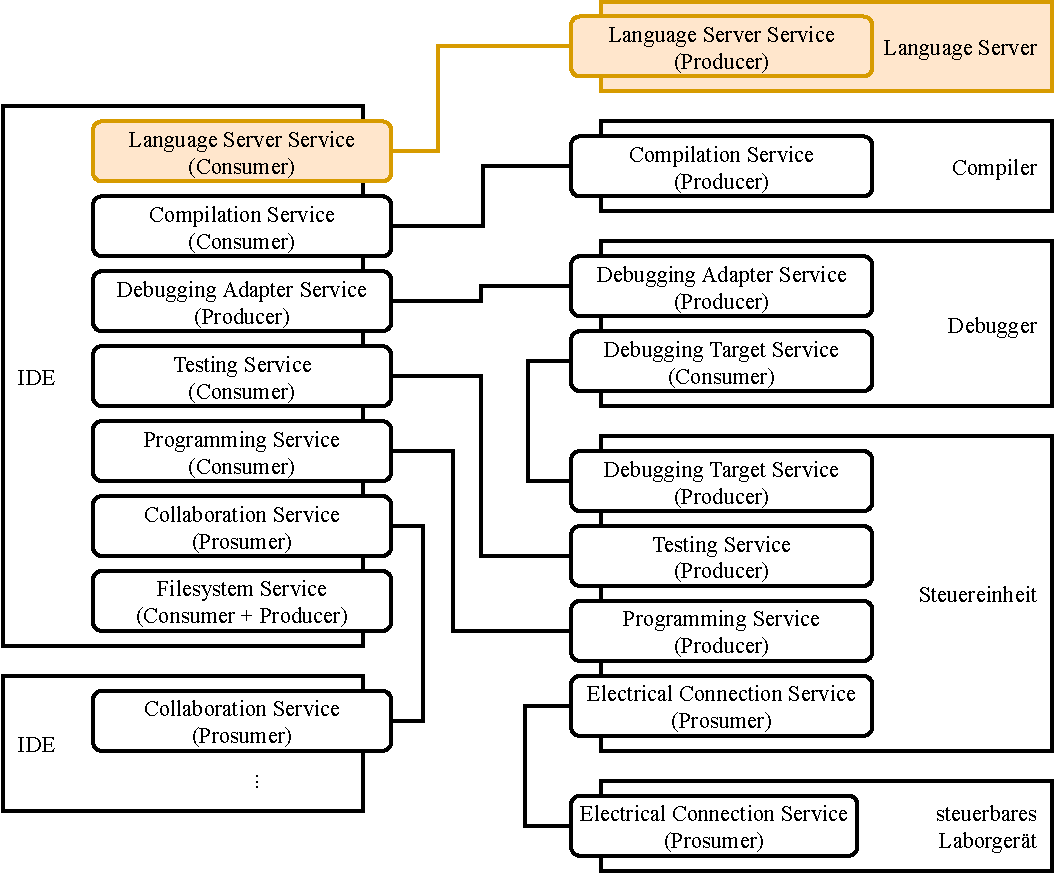
\includegraphics[width=\textwidth]{diagrams/experimentkonfigurationen/Experimentkonfiguration-06.drawio.pdf}
    \caption{Experimentkonfiguration (+ Language Server)}
    \label{figure:experimentkonfiguration:language-server}
\end{figure}